%4.2	Alternativas de diseño 
%Describir alternativas de diseño consideradas y las razones usadas para elegir la alternativa finalmente escogida.
\section{Design Alternatives}
%Guante & Flystick & Voice Recognition
%3D Joystick ->2D Joystick + Slider
The goal of this section is to explain the design alternatives and the reasons behind the selection of the alternative that was ultimately implemented. Even in the case that there weren't alternatives at all, like in the system architecture, this section will still explain the pros and cons of the default design.
\subsection{System Architecture}
The system running the application is a three-layered system, as can bee seen in the image below . The top level, the VRPN Tracking servers receives tracking information from the tablet VRPN device, which design will be discussed later, and from the IR tracking cameras following the flat passive markers attached to the back of the tablet.

\begin{center}
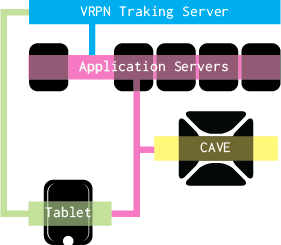
\includegraphics[scale=0.75]{Images/architecture.png}
\label{fig:architecture}
\end{center}

The VRPN server centralizes and retransmit the information from all the interaction devices that interact with the immersive system in which are used, in this case the tablet and the passive stereo glasses. The use of VRPN was a must for the project, as shown by the Non Functional Requirements in the previous chapter. VRPN stands for \emph{Virtual Reality Peripheral Network} and is ``... a set of classes within a library and a set of servers that implement a device-independent, network-transparent interface between application programs and the set of physical devices (trackers, buttons, etc.) used in a virtual reality (VR) system'' as defined by its creators in \cite{vrpn}. The use of VRPN is a development standar at the Institute Image as well as at the COLIVRI laboratory because of the flexibility provided by an abstraction level that separates front-end devices from the application input.

The second layer is composed by the Application Servers in charge of rendering the scene to project it in the Cave. One of these application servers render the scene from the tablet point of view, and stream the scene in real time, to allow the camera metaphor that will be explained in the User Interaction section of this chapter. Is important to note, that there isn't communication between those servers; each one, renders the scene from a particular perspective calculating the adequate frustrum for it's designated screen. Each of the Application Servers renders the images for both eyes of it's screen, but each image is projected by a different projector in order to work as a passive 3D system.
\subsection{User Interaction}
\subsubsection{Front-end Device}
\subsubsection{Application Workflow}
\subsubsection{User Interface}

\subsection{Software}
\subsubsection{Cave}
\subsubsection{Tablet}
